\documentclass[12pt,a4paper]{article}
    \usepackage[T2A]{fontenc}
    \usepackage[utf8]{inputenc}
    \usepackage[russian]{babel}
    \usepackage{amsmath}
    \usepackage{amssymb}
    \usepackage{graphicx}
    \usepackage{floatrow}
    \usepackage{booktabs}
    \usepackage{wrapfig}
    \usepackage{lipsum}
    \usepackage{subcaption}
    \usepackage{fancyhdr}
    \usepackage{mathrsfs}
    \usepackage{tikz}

    \usepackage{graphicx, scalerel}
    \usepackage[warn]{mathtext}
    \usepackage{indentfirst}
    \usepackage[margin = 25mm]{geometry}
    \usepackage{caption}
    \usepackage{multirow}
    \usepackage{gensymb}
    
    \newcommand{\figref}[1]{(См. рис. \ref{#1})}
    \newcommand{\secref}[1]{(См. раздел. \ref{#1})}
    
    \newcommand{\e}[1]{\text{$\cdot10^{#1}$}}
    
    \pagestyle{fancy}
    \fancyhead{}
    \fancyhead[L]{Работа 5.1.2}
    \fancyhead[R]{}
    \fancyfoot[C]{\thepage}
    
    \author{\normalsize Выполнил: Голубович Тимур, группа Б01-110 \\
    	\normalsize 01.11.2023}
    \date{}

    \usepackage{float}
    \restylefloat{table}
    \title{
    	\large Отчет о выполнении лабораторной работы 5.5.5 \\
    	\Large Компьютерная сцинтилляционная $\gamma$-спектрометрия
     }

    \begin{document}
\maketitle

\section*{Цель работы}

В данной работе предполагается изучить спектр гамма-излучений для образцов $ \mathrm{^{22}Na, ^{137}Cs, ^{60}Co, ^{241}Am \;} \text{и} \mathrm{\; ^{152}Eu}$, найти для них пики полного поглощения и обратного рассеяния.

\section*{Оборудование и приборы}

Источник  $\gamma$-квантов со свинцовым коллиматором; набор поглотителей из различных материалов; сцинтилляционныйй счётчик; пересчётный прибор.
	
\section*{Теоретическое введение}

Основная задача спектрометрических измерений заключается в определении энергии, интенсивности дискретных гамма-линий от различных гамма-источников и их идентификации.
	
Основными процессами взаимодействия гамма-излучения с веществом являются фотоэффект, эффект Комптона и образование электрон-позитронных пар. Каждый из этих процессов вносит свой вклад в образование наблюдаемого спектра. Образующиеся при этих процессах электроны испытывают большое количество неупругих соударений с молекулами и атомами среды. Неупругие соударения могут сопровождаться как ионизацией, так и возбуждением молекул или атомов среды. В промежуточных же стадиях (при переходах возбужденных молекул или атомов в основное состояние, при рекомбинации электрических зарядов и т.п.) в веществе возникают кванты света различных длин волн, присущих данному веществу.
	
При \textbf{фотоэффекте} кинетическая энергия электрона $ T_e = E_{\gamma} - I_i $, где $ I_i $ --- энергия ионизации $ i $-той оболочки атома. Фотоэффект особенно существенен для тяжелых веществ, где он идет с заметной вероятностью даже при высоких энергиях гамма-квантов. В легких веществах фотоэффект становится заметен лишь при относительно небольших энергиях гамма-квантов. Наряду с фотоэффектом, при котором вся энергия гамма-кванта передается атомному электрону, взаимодействие гамма-излучения со средой может приводить к его рассеянию, т.е. отклонению от первоначального направления распространения на некоторый угол.
	
При \textbf{эффекте Компотна} происходит упругое рассеяние фотона на свободном электроне, сопровождающееся изменением длины волны фотона (реально этот процесс происходит на слабо связанных с атомом внешних электронах). Максимальная энергия образующихся комптоновских электронов соответствует рассеянию гамма-квантов на $ 2\pi $ и равна
	
\begin{equation}\label{E_compton}
	E_{c \_ max} = \dfrac{\hbar \omega}{1 + \dfrac{m_ec^2}{2\hbar\omega}}
\end{equation}
	
При достаточно высокой энергии гамма-кванта наряду с фотоэффектом и эффектом Комптона может происходить третий вид взаимодействия гамма-квантов с веществом – \textbf{образование электрон-позитронных пар}. При этом если процесс образования пары идет в кулоновском поле ядра или протона, то энергия образующегося ядра отдачи оказывается весьма малой, так что пороговая энергия гамма-кванта, необходимая для образования пары, практически совпадает с удвоенной энергией покоя электрона $ E_0 = 2m_ec^2 = 1.022  $МэВ.
	
Появившийся в результате процесса образования пар электрон теряет свою энергию на ионизацию среды. Таким образом, вся энергия электрона остается в детекторе. Позитрон будет двигаться до тех пор, пока практически не остановится, а затем аннигилирует с электроном среды, в результате чего появятся два гамма-кванта. Т.е., кинетическая энергия позитрона также останется в детекторе. Далее возможны три варианта развития событий:
	
а) оба родившихся гамма-кванта не вылетают из детектора, и тогда вся энергия первичного гамма-кванта останется в детекторе, а в спектре появится пик с $ E = E_\gamma $;
	
б) один из родившихся гамма-квантов покидает детектор, и в спектре появляется пик, соответствующий энергии $ E = E_\gamma - E0 $, где $ E_0 = m_ec^2 = $ 511 кэВ;
	
в) оба родившихся гамма-кванта покидают детектор, и в спектре появля- ется пик, соответствующий энергии $ E = E_\gamma - 2E0 $, где $ 2E_0 = 2m_ec^2 = $ 1022 кэВ;
	
Таким образом, любой спектр, получаемый с помощью гамма-спектрометра, описывается несколькими компонентами, каждая из которых связана с определенным физическим процессом. Как описано выше, основными физическими процессами взаимодействия гамма-квантов с веществом являются фотоэффект, эффект Комптона и образование электрон-позитронных пар, и каждый из них вносит свой вклад в образование спектра. Помимо этих процессов, добавляются экспонента, связанная с наличием фона, пик характеристического излучения, возникающий при взаимодействии гамма-квантов с окружающим веществом, а также пик обратного рассеяния, образующийся при энергии квантов $ E_\gamma \gg mc^22/2 $ в результате рассеяния гамма-квантов на большие углы на материалах конструктивных элементов детектора и защиты. Положение пика обратного рассеяния определяется по формуле ($ E $ --- энергия фотопика):
	
\begin{equation}\label{Eobr}
	E_{\text{обр}} = \dfrac{E}{1 + \dfrac{2E}{mc^2}}
\end{equation}
 	
 
\section*{Экспериментальная установка}
	
Энергетическим разрешением спектрометра называется величина
	
\begin{equation}\label{Ri = dE/E}
	R_i = \dfrac{\Delta E_i}{E_i}
\end{equation}
	
т.е. отношение ширины пика полного поглощения (измеренной на полувысоте) к регистрируемой энергии пика поглощения. Это значение $ E_i \propto \overline{n_i} $ --- числу частиц на выходе ФЭУ. При этом  $ \Delta E_i \propto \overline{\Delta n_i} = \sqrt{\overline{n_i}} $ --- ширина пика пропорциональна среднеквадратичной флуктуации, которая равна корню из числа частиц. Таким образом, наша формула \eqref{Ri = dE/E} примет вид
	
\begin{equation}\label{Ri = c/E}
	R_i = \dfrac{\mathrm{const}}{\sqrt{E_i}}
\end{equation}

\begin{figure}[h!]
    \centering
 	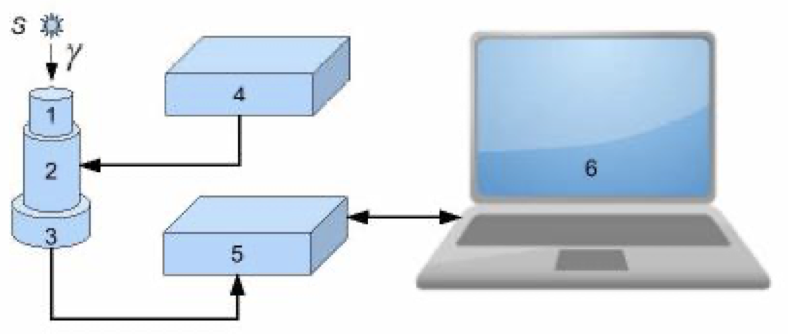
\includegraphics[width=\linewidth]{res/scheme.png}
 	\caption{Экспериментальная установка}
 	\label{Scheme_Compton}
\end{figure}

\section*{Ход работы}

Проведем измерения гамма-спектров для $ \mathrm{^{22}Na, ^{137}Cs, ^{60}Co, ^{241}Am \;} \text{и} \mathrm{\; ^{152}Eu}$, а также измерение фона. Измерения для цезия повторим на соседней установке. Получаем зависимость счета на сцинтилляторе $ N'_\text{ч} $ от номера канала $ N $. 
	
Найдем пики полного рассеяния для натрия $ \mathrm{^{22}Na} $ и цезия $ \mathrm{^{137}Cs} $:
	
\begin{equation}\label{}
	N_{Na\_1} = 597.5, \quad N_{Na\_2} = 1395.2, \quad N_{Cs} =754.2
\end{equation}
	
Мы знаем, что этим пикам соответствуют табличные значения энергии 511, 1275 и 662 кэВ соответственно. Тогда проведем калибровку спектрометра, построив линейную зависимость энергии гамма-кванта от номера канала $ E_j = f(N_j) $. Результат калибровки:
	
\begin{equation}\label{}
	E_j = (-60.537 + 0.957N_i ) \; \text{кэВ}
\end{equation}
	
С помощью полученной зависимости переведем все полученные значения каналов в энергии, а счет сцинтиллятора отнормируем по времени, получив число частиц за секунду $ N_\text{ч} = \dfrac{N'_\text{ч}}{t} $. Погрешность счета подсчитаем по формуле 

\begin{equation}\label{}
	\sigma_{N_\text{ч}} = N_\text{ч} \cdot \dfrac{\sqrt{N'_\text{ч}}}{N'_\text{ч}} = \dfrac{\sqrt{N'_\text{ч}}}{t}
\end{equation}
	
Во всех измерениях $ t $ в диапазоне 600 -- 700 секунд. Отложим по оси абсцисс энергию полученных экспериментальных точек, а по оси ординат -- число частиц за секунду (рис. 1 -- 6).
	
С помощью ПО компьютера экспериментальной установки получим значения пиков полного поглощения и их ширины. По формуле \eqref{Ri = dE/E} подсчитаем для них разрешающую способность спектрометра. Результаты сведем в таблицу.
	
\begin{figure}[H]
	\label{graf_bg}
	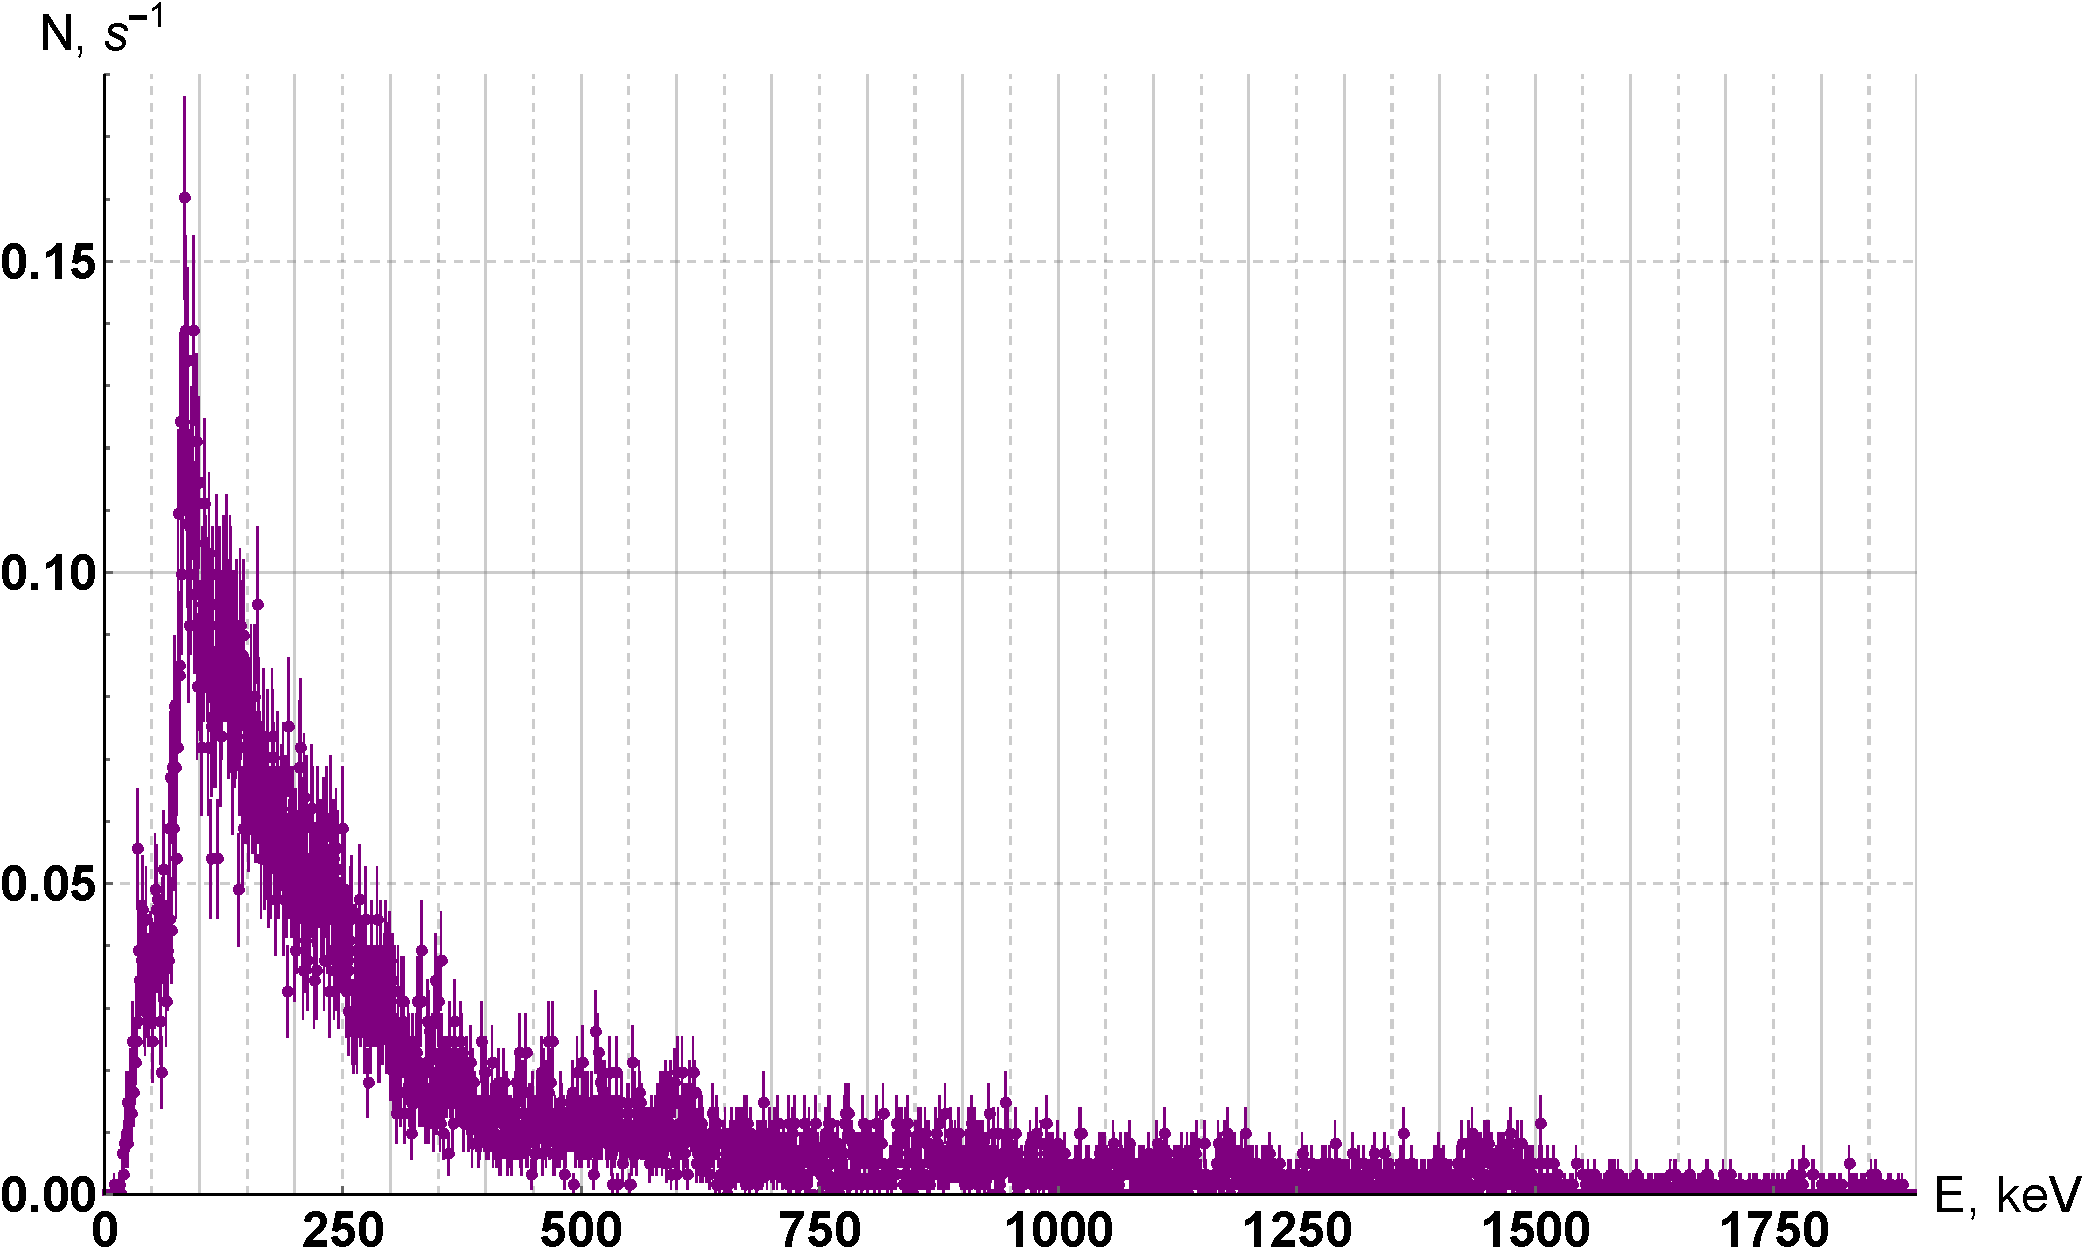
\includegraphics[width=10cm]{src/bg.pdf}
	\caption{Измерение фона}
\end{figure} 	
	
\begin{figure}[H]
	\label{graf_na}
	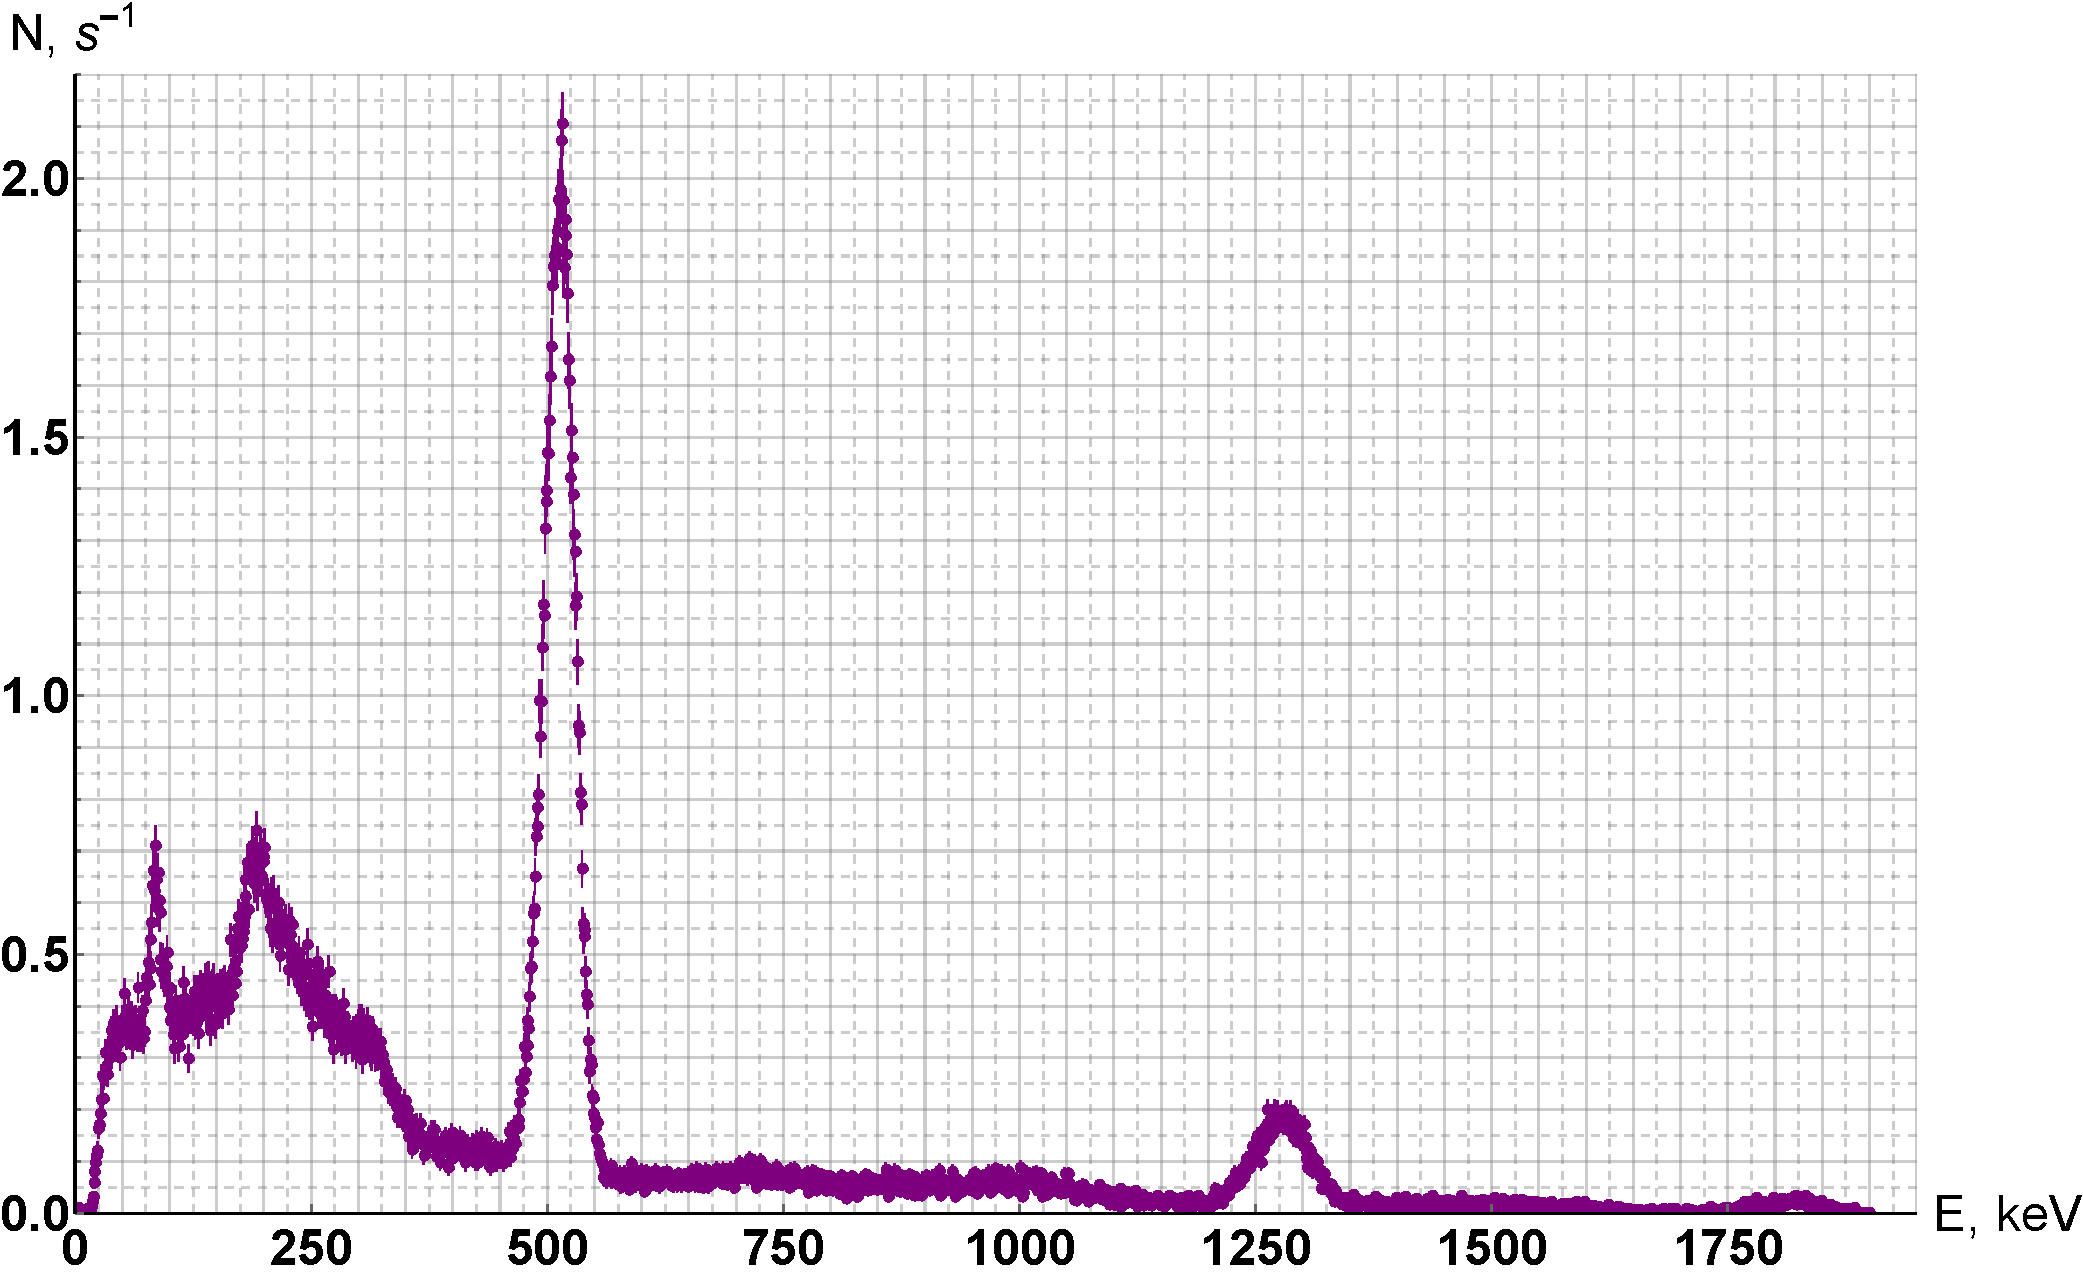
\includegraphics[width=10cm]{src/na.pdf}
	\caption{Измерение спектра источника натрия $ \mathrm{^{22}Na} $}
\end{figure} 

\begin{figure}[H]
	\label{graf_co}
	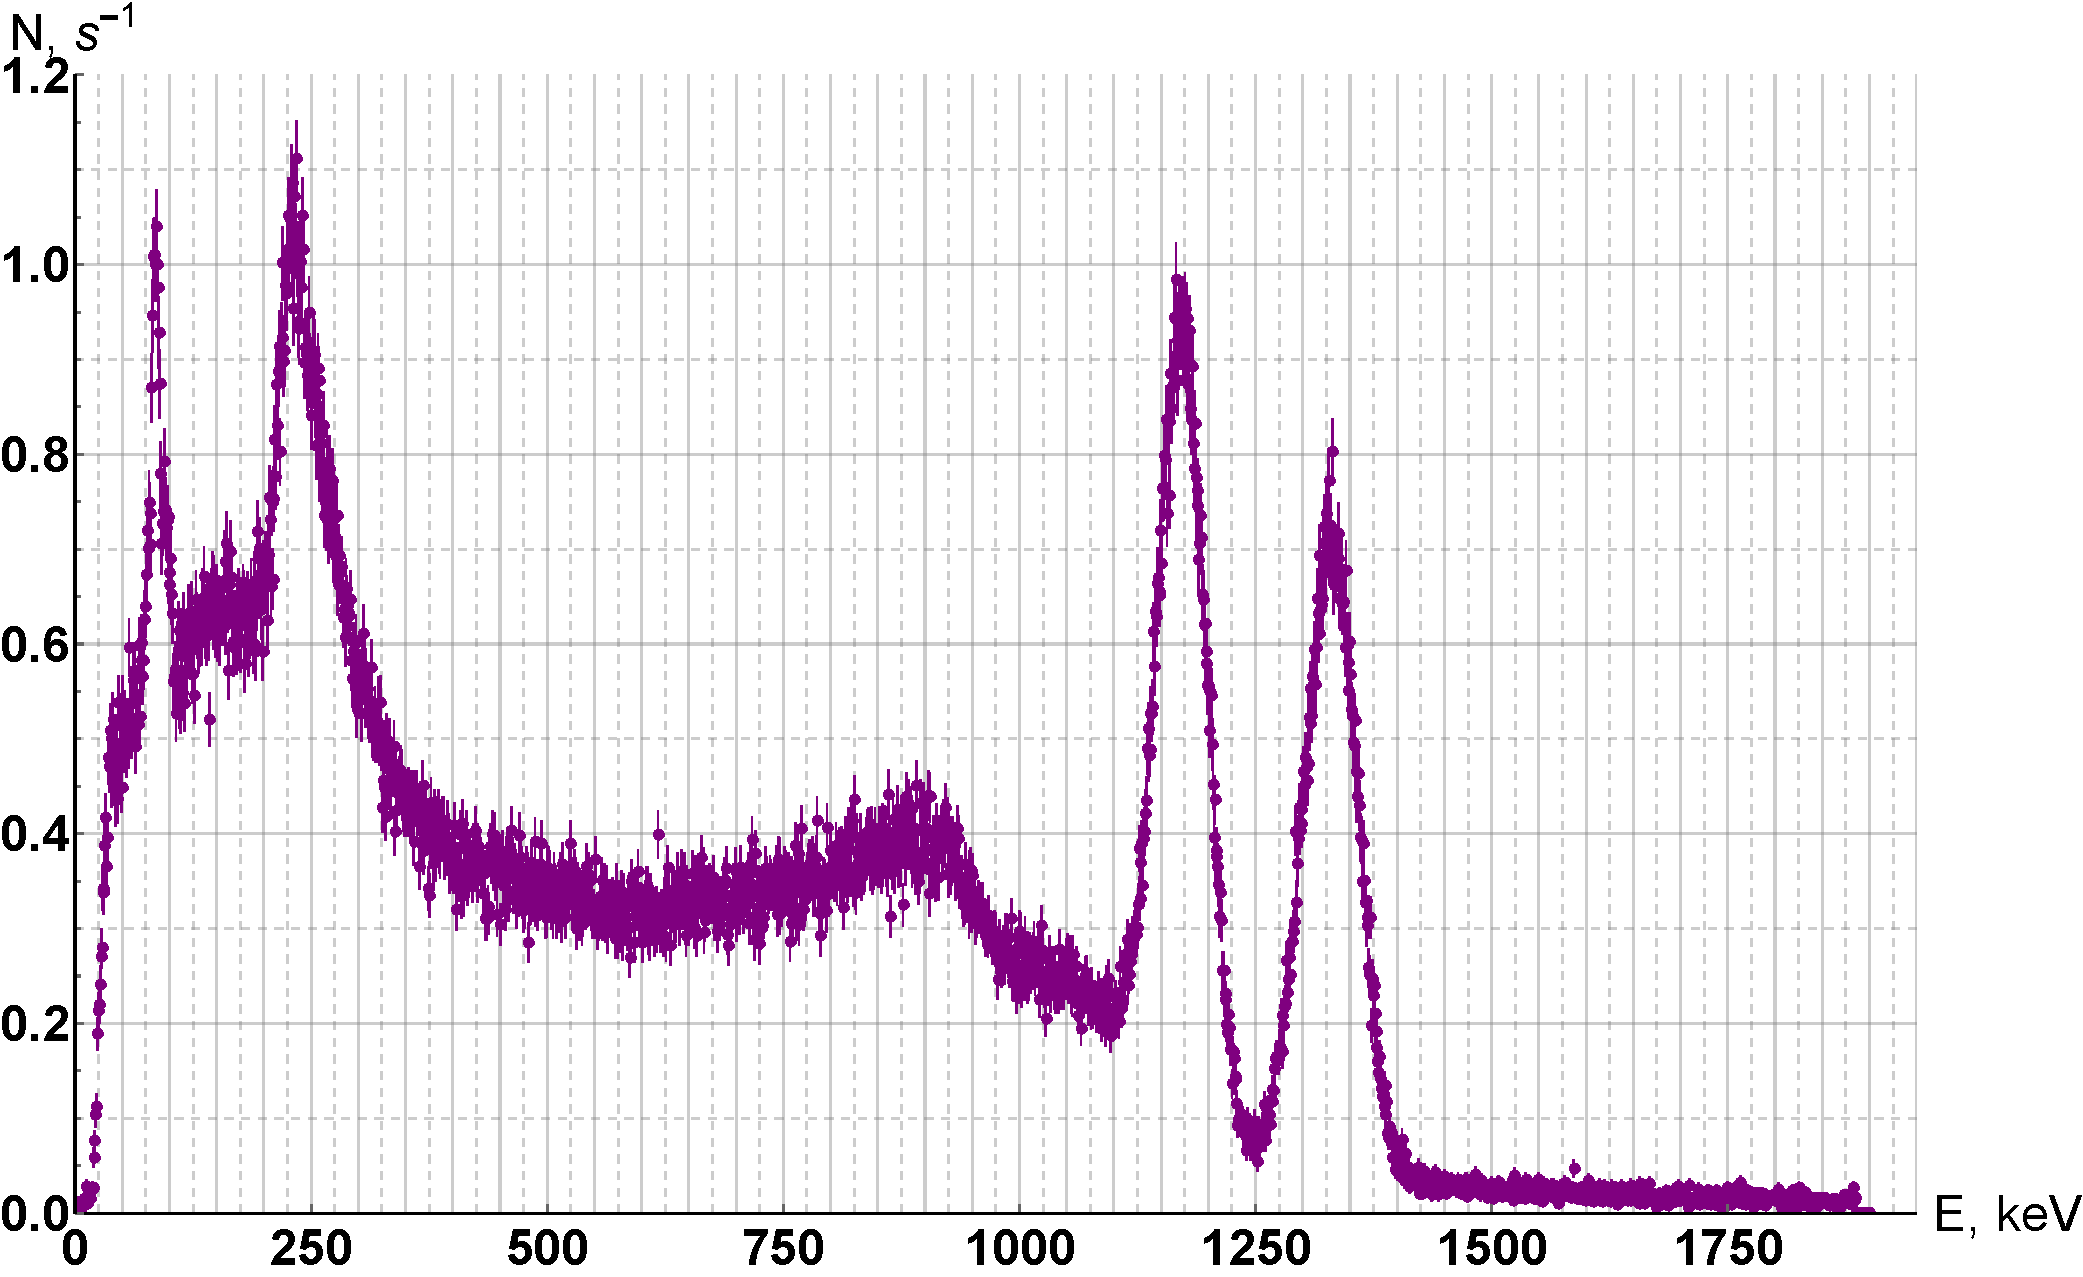
\includegraphics[width=10cm]{src/co.pdf}
	\caption{Измерение спектра источника кобальта $ \mathrm{^{60}Co} $}
\end{figure} 
    
\begin{figure}[H]
	\label{graf_cs}
	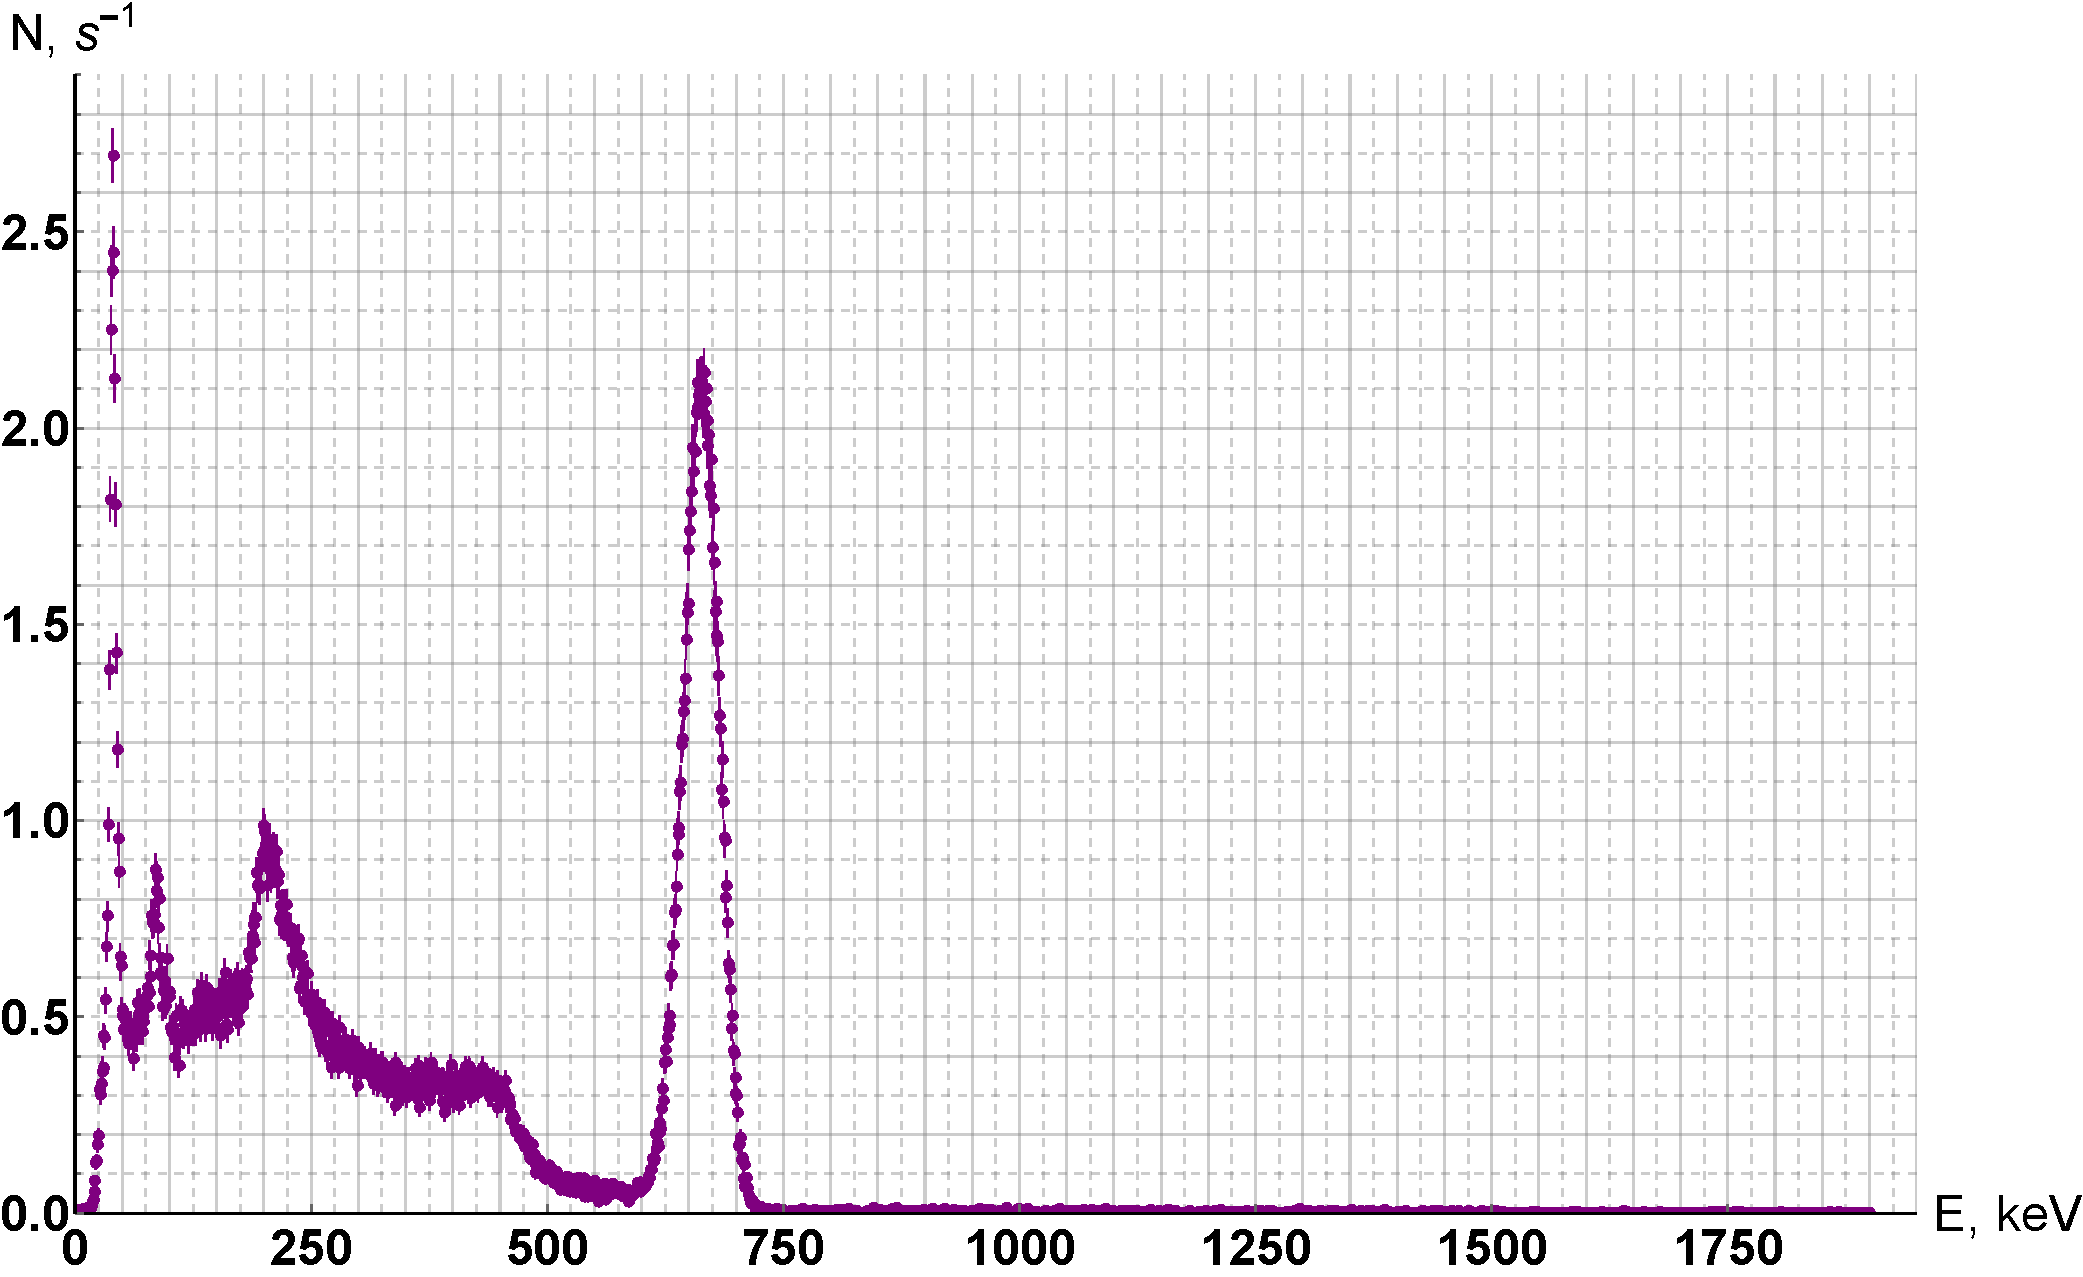
\includegraphics[width=10cm]{src/cs.pdf}
	\caption{Измерение спектра источника цезия $ \mathrm{^{137}Cs} $}
\end{figure} 
    
\begin{figure}[H]
	\label{graf_cs2}
	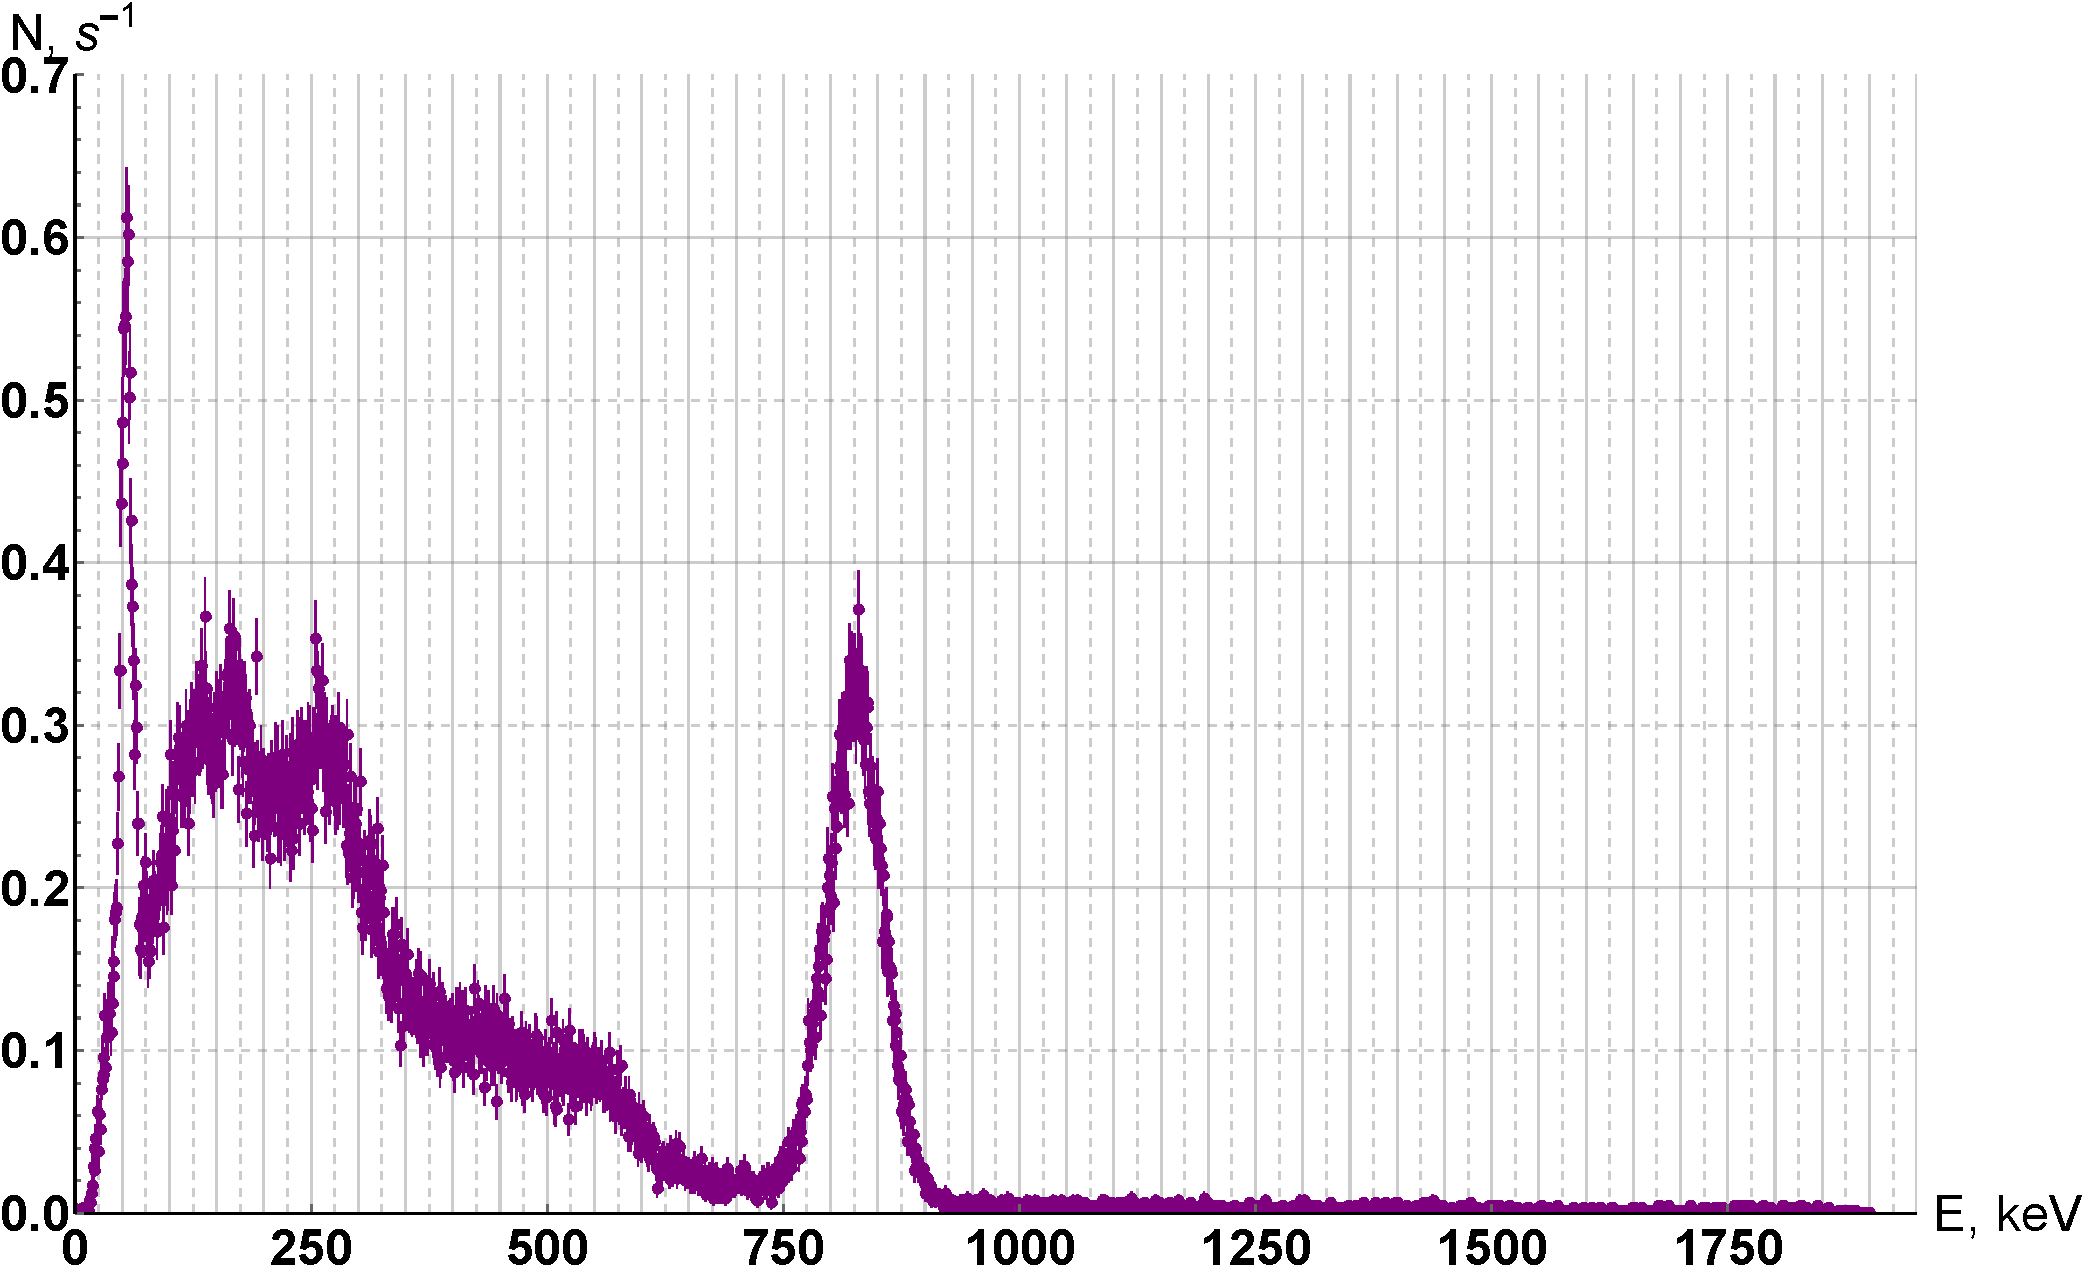
\includegraphics[width=10cm]{src/cs2.pdf}
	\caption{Измерение на второй установке спектра источника цезия $ \mathrm{^{137}Cs} $} 
\end{figure} 
    
\begin{figure}[H]
	\label{graf_am}
	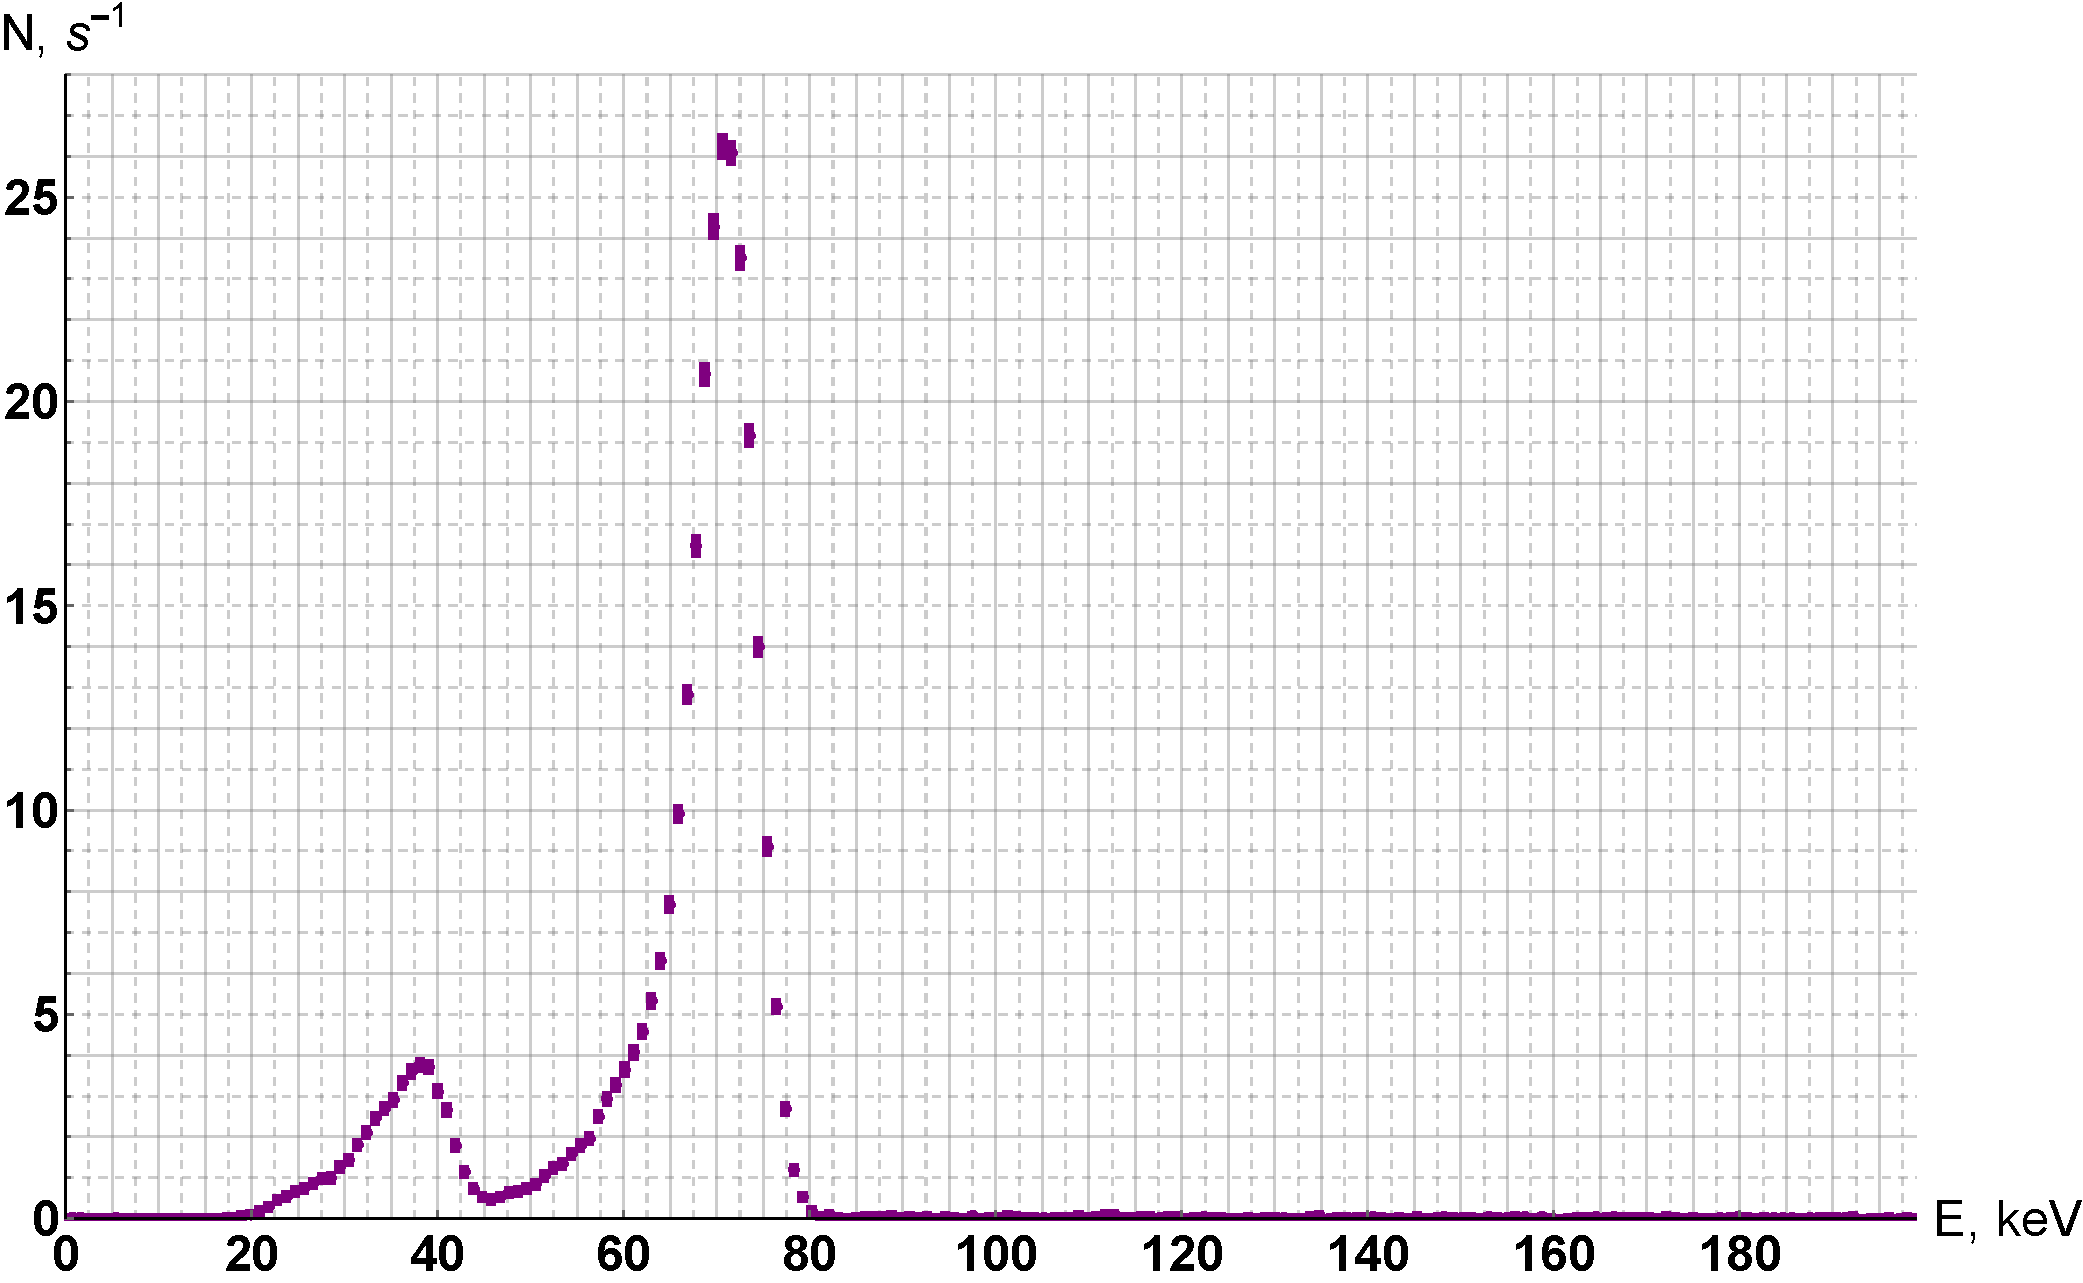
\includegraphics[width=10cm]{src/am.pdf}
	\caption{Измерение спектра источника америция $ \mathrm{^{241}Am} $}
\end{figure} 
    
\begin{figure}[H]
	\label{graf_eu}
	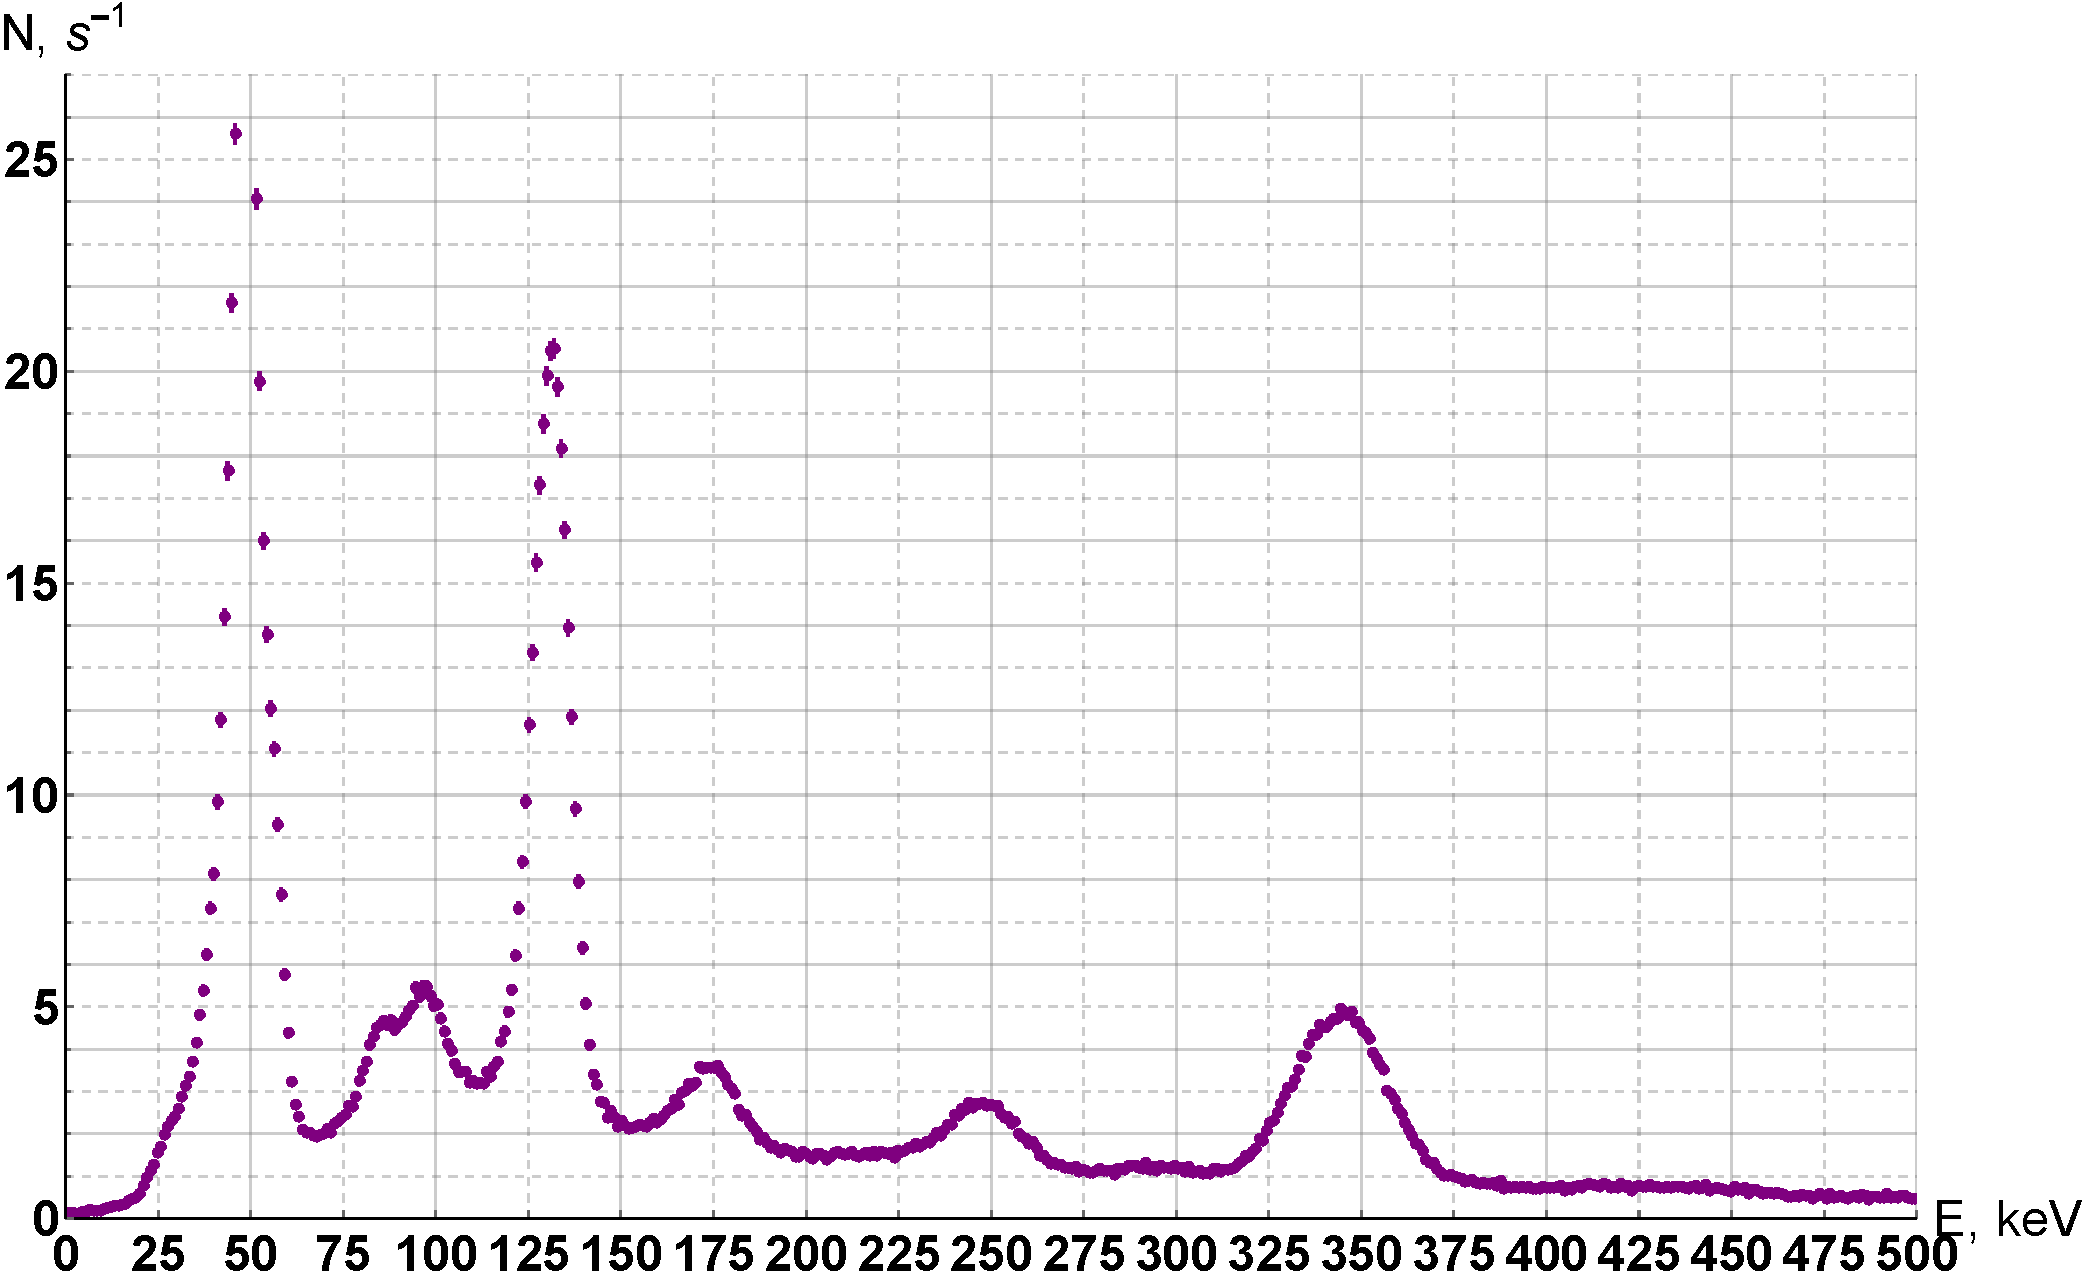
\includegraphics[width=10cm]{src/eu.pdf}
	\caption{Измерение спектра источника европия $ \mathrm{^{152}Eu} $}
\end{figure}

\begin{table}[H]
	\caption{Пики прямого поглощения}
	\begin{center}
		\begin{tabular}{|c|c|c|c|c|c|}
			\hline 
			Образец                         & $N_i $  & $ \Delta N_i $ & $ E_i, $ кэВ & $ \Delta E,_i $ кэВ & $ R_i $ \\ 
			\hline 
			Натрий $ \mathrm{^{22}Na} $      & 597.48  & 42             & 511.4           & 40.2                   & 0.079   \\
			Натрий $ \mathrm{^{22}Na} $      & 1395.23 & 76.6           & 1275.1          & 73.4                   & 0.058   \\
			Цезий $ \mathrm{^{137}Cs} $       & 754.22  & 47.4           & 661.5           & 45.3                   & 0.069   \\
			Кобальт $ \mathrm{^{60}Co} $    & 1286.1  & 65.1           & 1170.6          & 62.3                   & 0.053   \\
			Кобальт $ \mathrm{^{60}Co} $    & 1450.59 & 73.3           & 1328.1          & 70.2                   & 0.053   \\
			Америций $ \mathrm{^{241}Am} $ & 135.57  & 9.5            & 69.2            & 9                      & 0.131   \\
			Европий	 $ \mathrm{^{152}Eu} $  & 199.01  & 12.3           & 130             & 11.7                   & 0.09    \\
			Европий	 $ \mathrm{^{152}Eu} $  & 320.8   & 23.1           & 246.6           & 22.1                   & 0.089   \\
			Европий	 $ \mathrm{^{152}Eu} $  & 421.7   & 30.4           & 343.2           & 29.1                   & 0.085   \\
							
			
			\hline 
		\end{tabular} 
	\end{center}
	\label{res}
\end{table}

Экспериментально оценим пики комптоновского рассеяния и сравним с теоретическим расчетом. Результаты сведем в таблицу. Построим график зависимости теоретического расчета от экспериментального. 
	
\begin{figure}[H]
	\label{graf_com}
	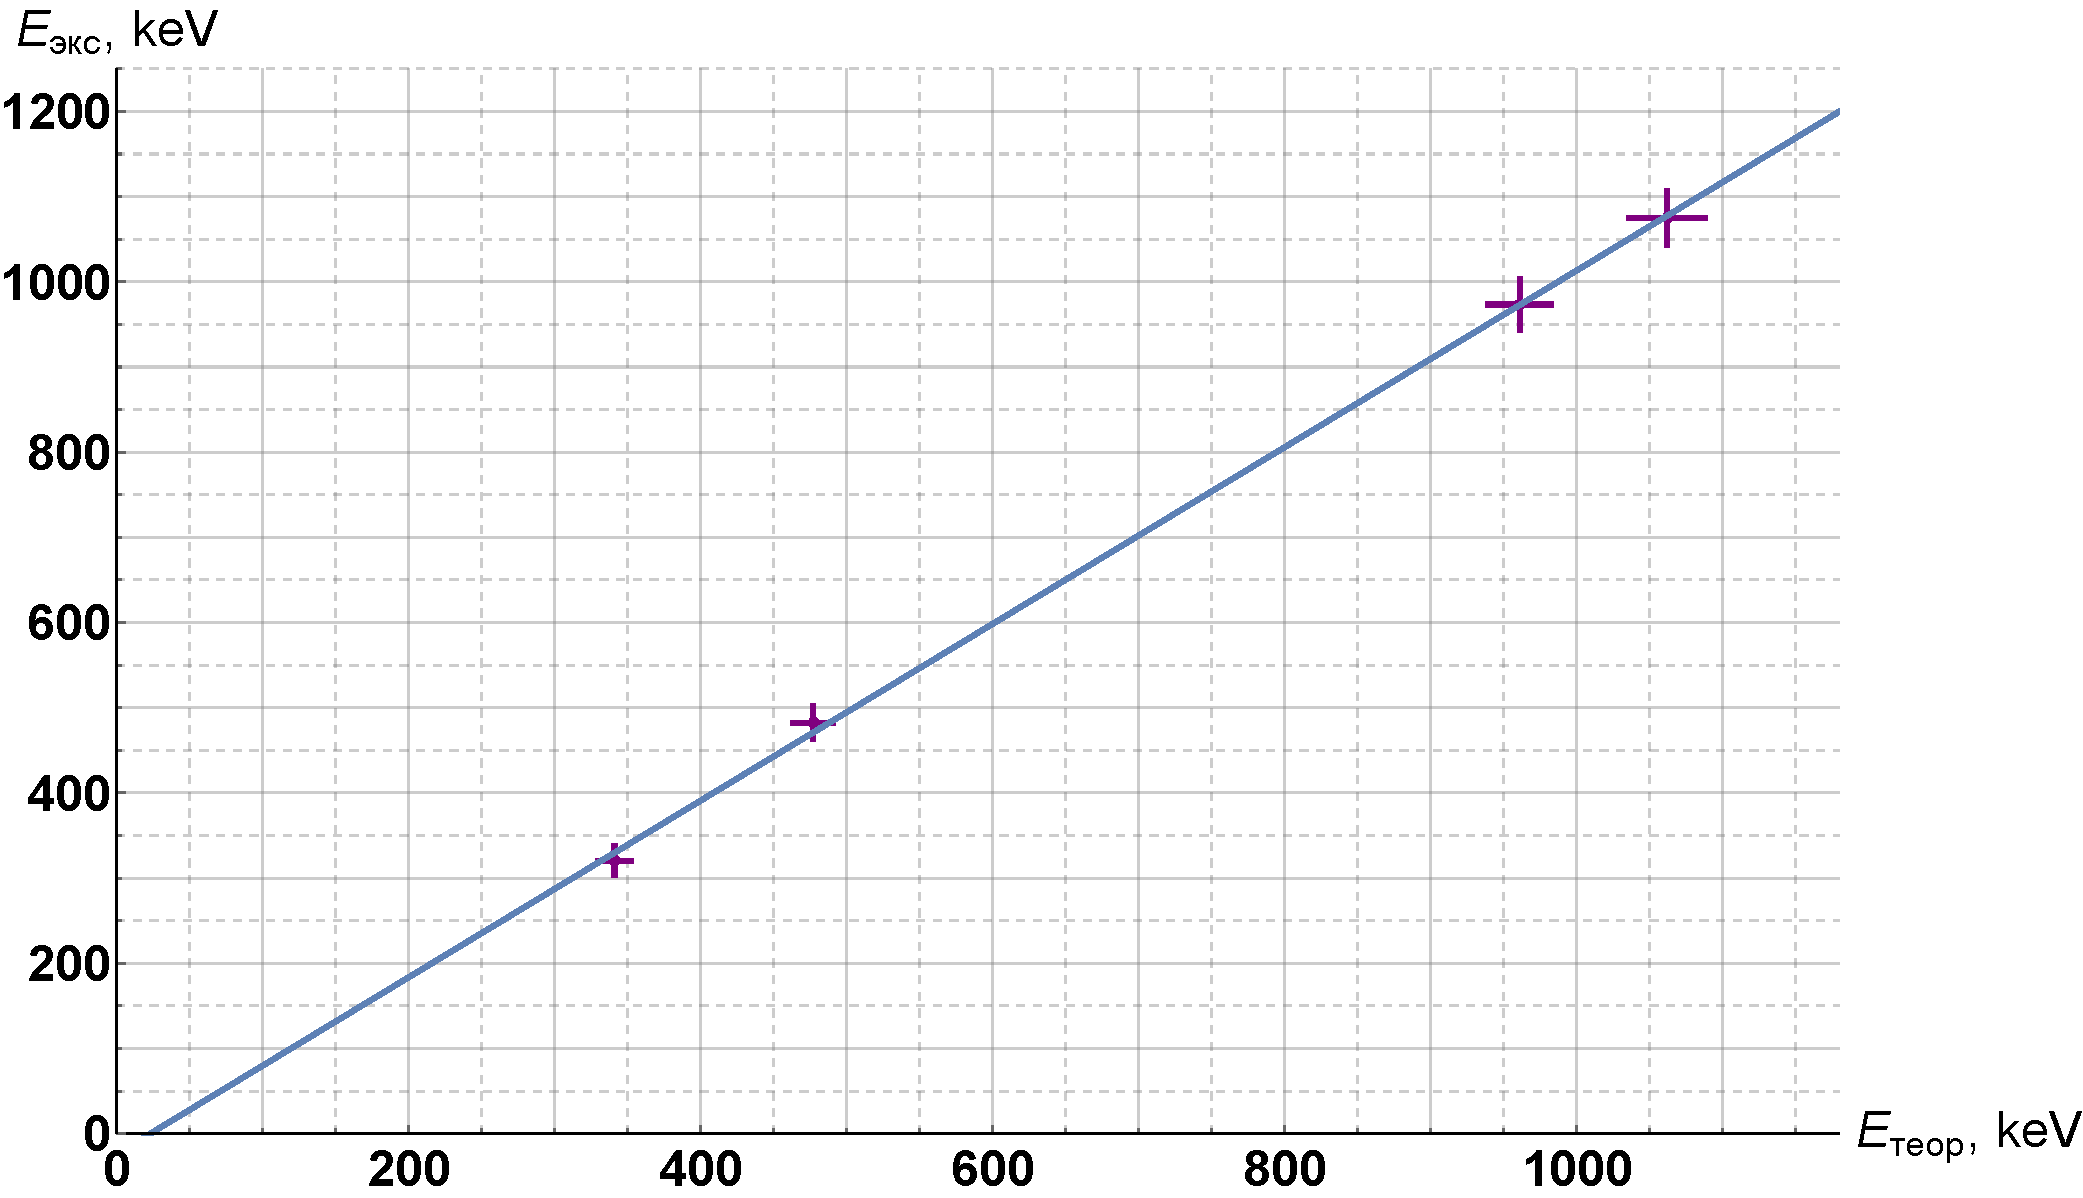
\includegraphics[width=10cm]{src/comp.pdf}
	\caption{Зависимости теоретического расчета края комптоновского спектра от экспериментального}
\end{figure} 
	
Найдем параметры фита: 


\begin{table}[H]
	\caption{Комптновские спектры}
	\begin{center}
		\begin{tabular}{|c|c|c|c|}
			\hline 
			Образец                      & $ E_i, $ кэВ & $ E_{c\; \text{экс}}, $ кэВ & $ E_{c \; \text{теор}}, $ кэВ \\
			\hline 
			Натрий $ \mathrm{^{22}Na} $   & 511.4           & 320.5                      & 341.                          \\
			Цезий $ \mathrm{^{137}Cs} $    & 661.5           & 482.2                      & 477.2                         \\
			Кобальт $ \mathrm{^{60}Co} $ & 1270.6          & 973.3                      & 960.9                         \\
			Натрий $ \mathrm{^{22}Na} $   & 1275.1          & 1075                       & 1062.3                        \\
			\hline 
		\end{tabular} 
	\end{center}
	\label{compt}
\end{table}

\begin{table}[H]
	\caption{Фит рис. 8 функцией $ y = ax + b $}
	\begin{center}
		\begin{tabular}{|c|c|c|}
			\hline
			  & \text{Estimate} & \text{Standard Error} \\
			\hline
			b & 23.43           & 12.36                 \\
			a & 0.96            & 0.02                  \\
			\hline 
		\end{tabular} 
	\end{center}
	\label{compt_fit}
\end{table}

Видим, что коэф. при $ x \simeq 1 $, т.е. результат согласуется с теорией. 


Для проверки соотношения \eqref{Ri = c/E} построим график зависимости $ R^2_i = f(\frac{1}{E_i}) $ для величин из таблицы 1. 
	
\begin{figure}[H]
	\label{graf_r2}
	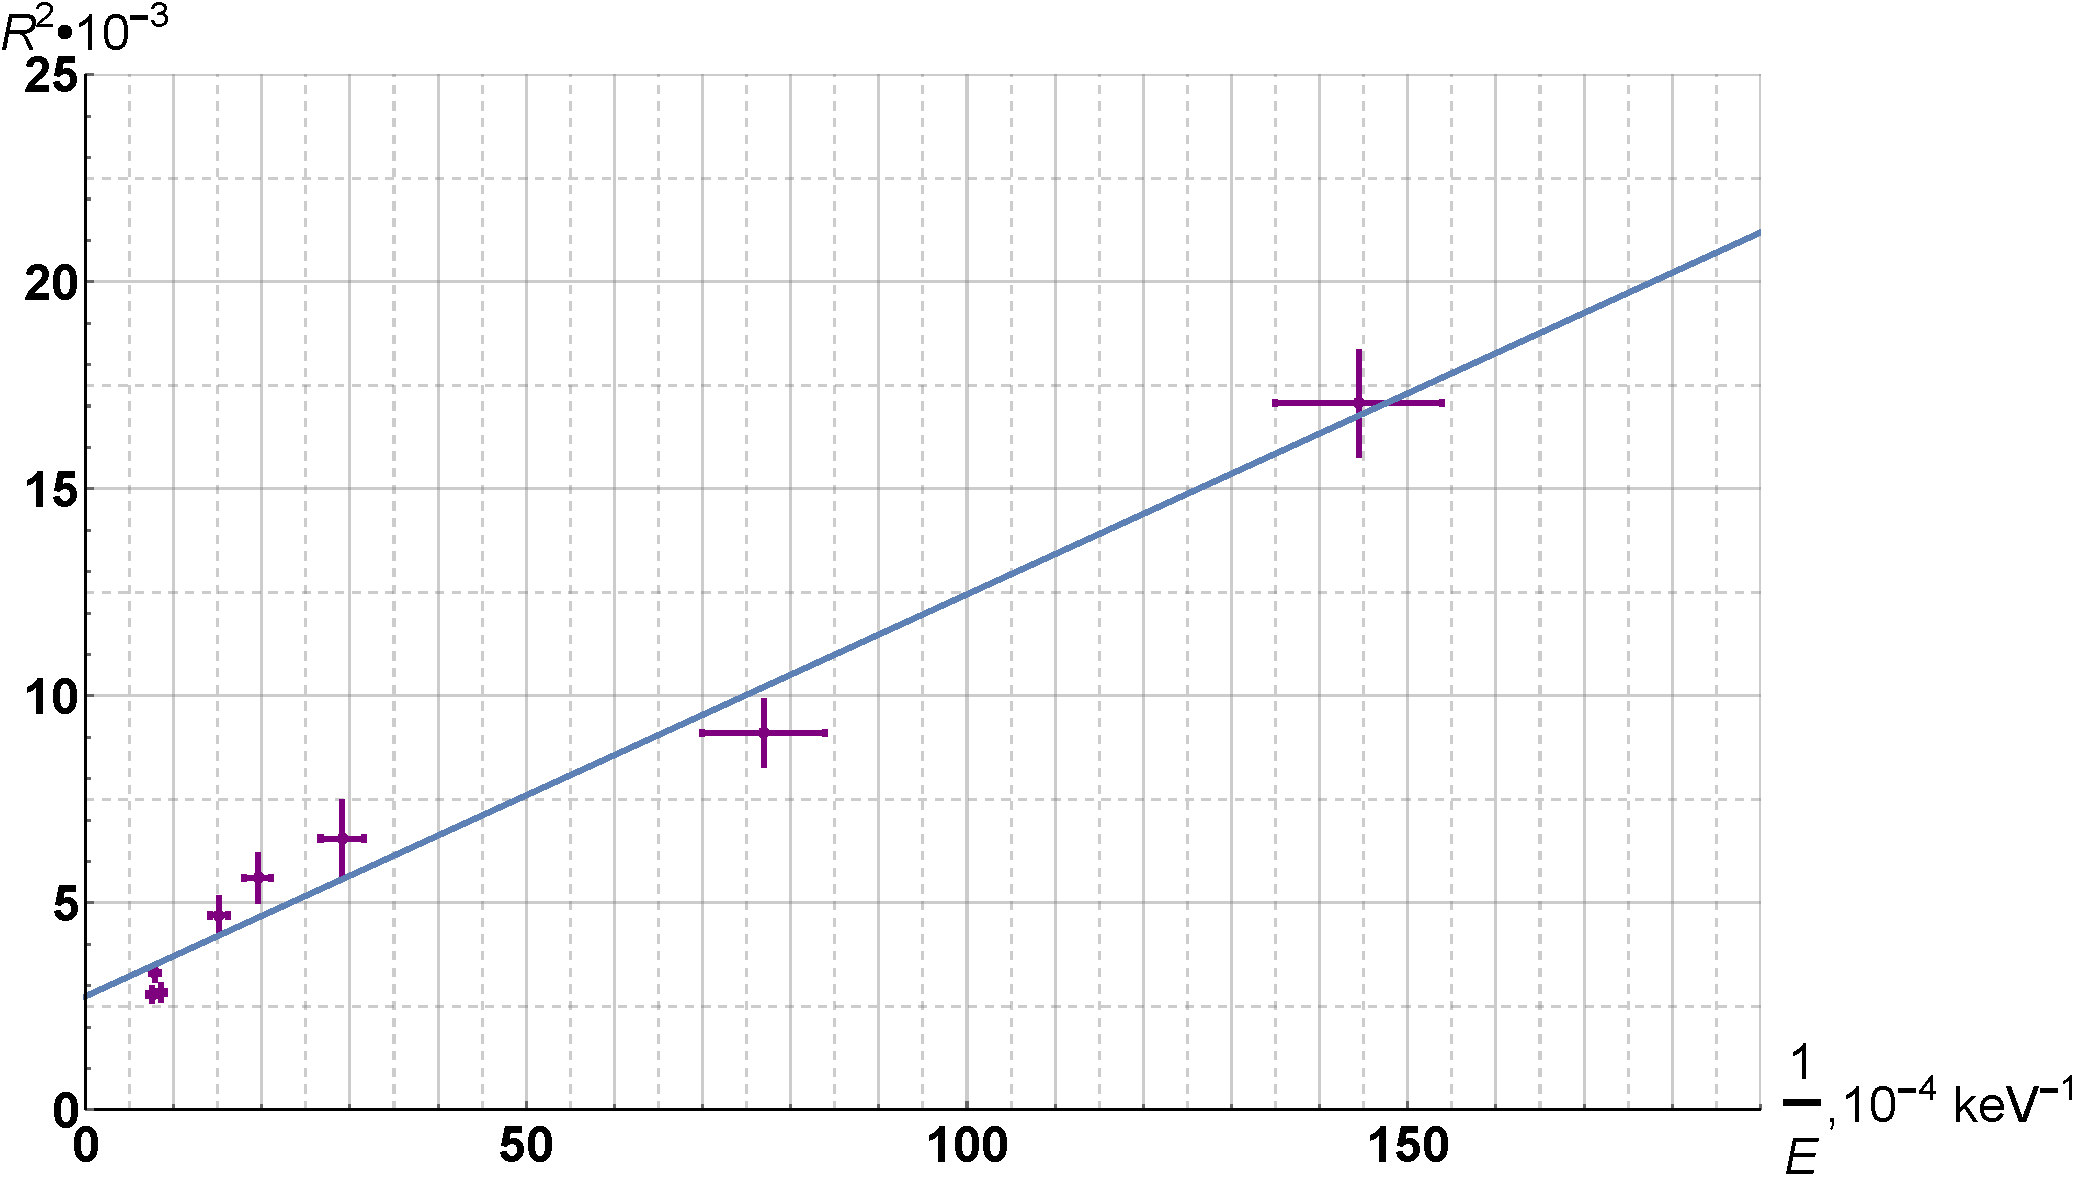
\includegraphics[width=10cm]{src/r^2.pdf}
	\caption{Проверка формулы $ R = \dfrac{\mathrm{const}}{\sqrt{E}} $}
\end{figure} 

Результаты фита сведем в таблицу:

\begin{table}[H]
	\caption{Фит рис. 9 функцией $ y = ax + b $}
	\begin{center}
		\begin{tabular}{|c|c|c|}
			\hline
			  & \text{Estimate} & \text{Standard Error} \\
			\hline
			b & 2.74367         & 0.40169               \\
			a & 0.097081        & 0.00673854            \\
			\hline 
		\end{tabular} 
	\end{center}
	\label{r2_fit}
\end{table}

Видно, что точки вполне хорошо описывают прямую.

Теперь найдем пики обратного рассеяния. 

\begin{table}[H]
	\caption{Пики обратного рассеяния}
	\begin{center}
		\begin{tabular}{|c|c|c|}
			\hline 
			Образец                        & $ E_i, $ кэВ & $ E_{\text{обр}}, $ кэВ \\
			\hline 
			Натрий $ \mathrm{^{22}Na} $     & 511.4           & 190                    \\
			Цезий $ \mathrm{^{137}Cs} $      & 661.5           & 205                    \\
			Кобальт $ \mathrm{^{60}Co} $   & 1328.1          & 230                    \\
			Европий	 $ \mathrm{^{152}Eu} $ & 129.973         & 95                     \\
			%			Европий	 $ \mathrm{^{152}Eu} $& 343.172 & 170 \\
			\hline 
		\end{tabular} 
	\end{center}
	\label{obr}
\end{table}

Построим график зависимости $ E_{\text{обр}} = f(E) $ согласно \eqref{Eobr} и нанесем экспериментальные точки:

\begin{figure}[H]
	\label{graf_obr}
	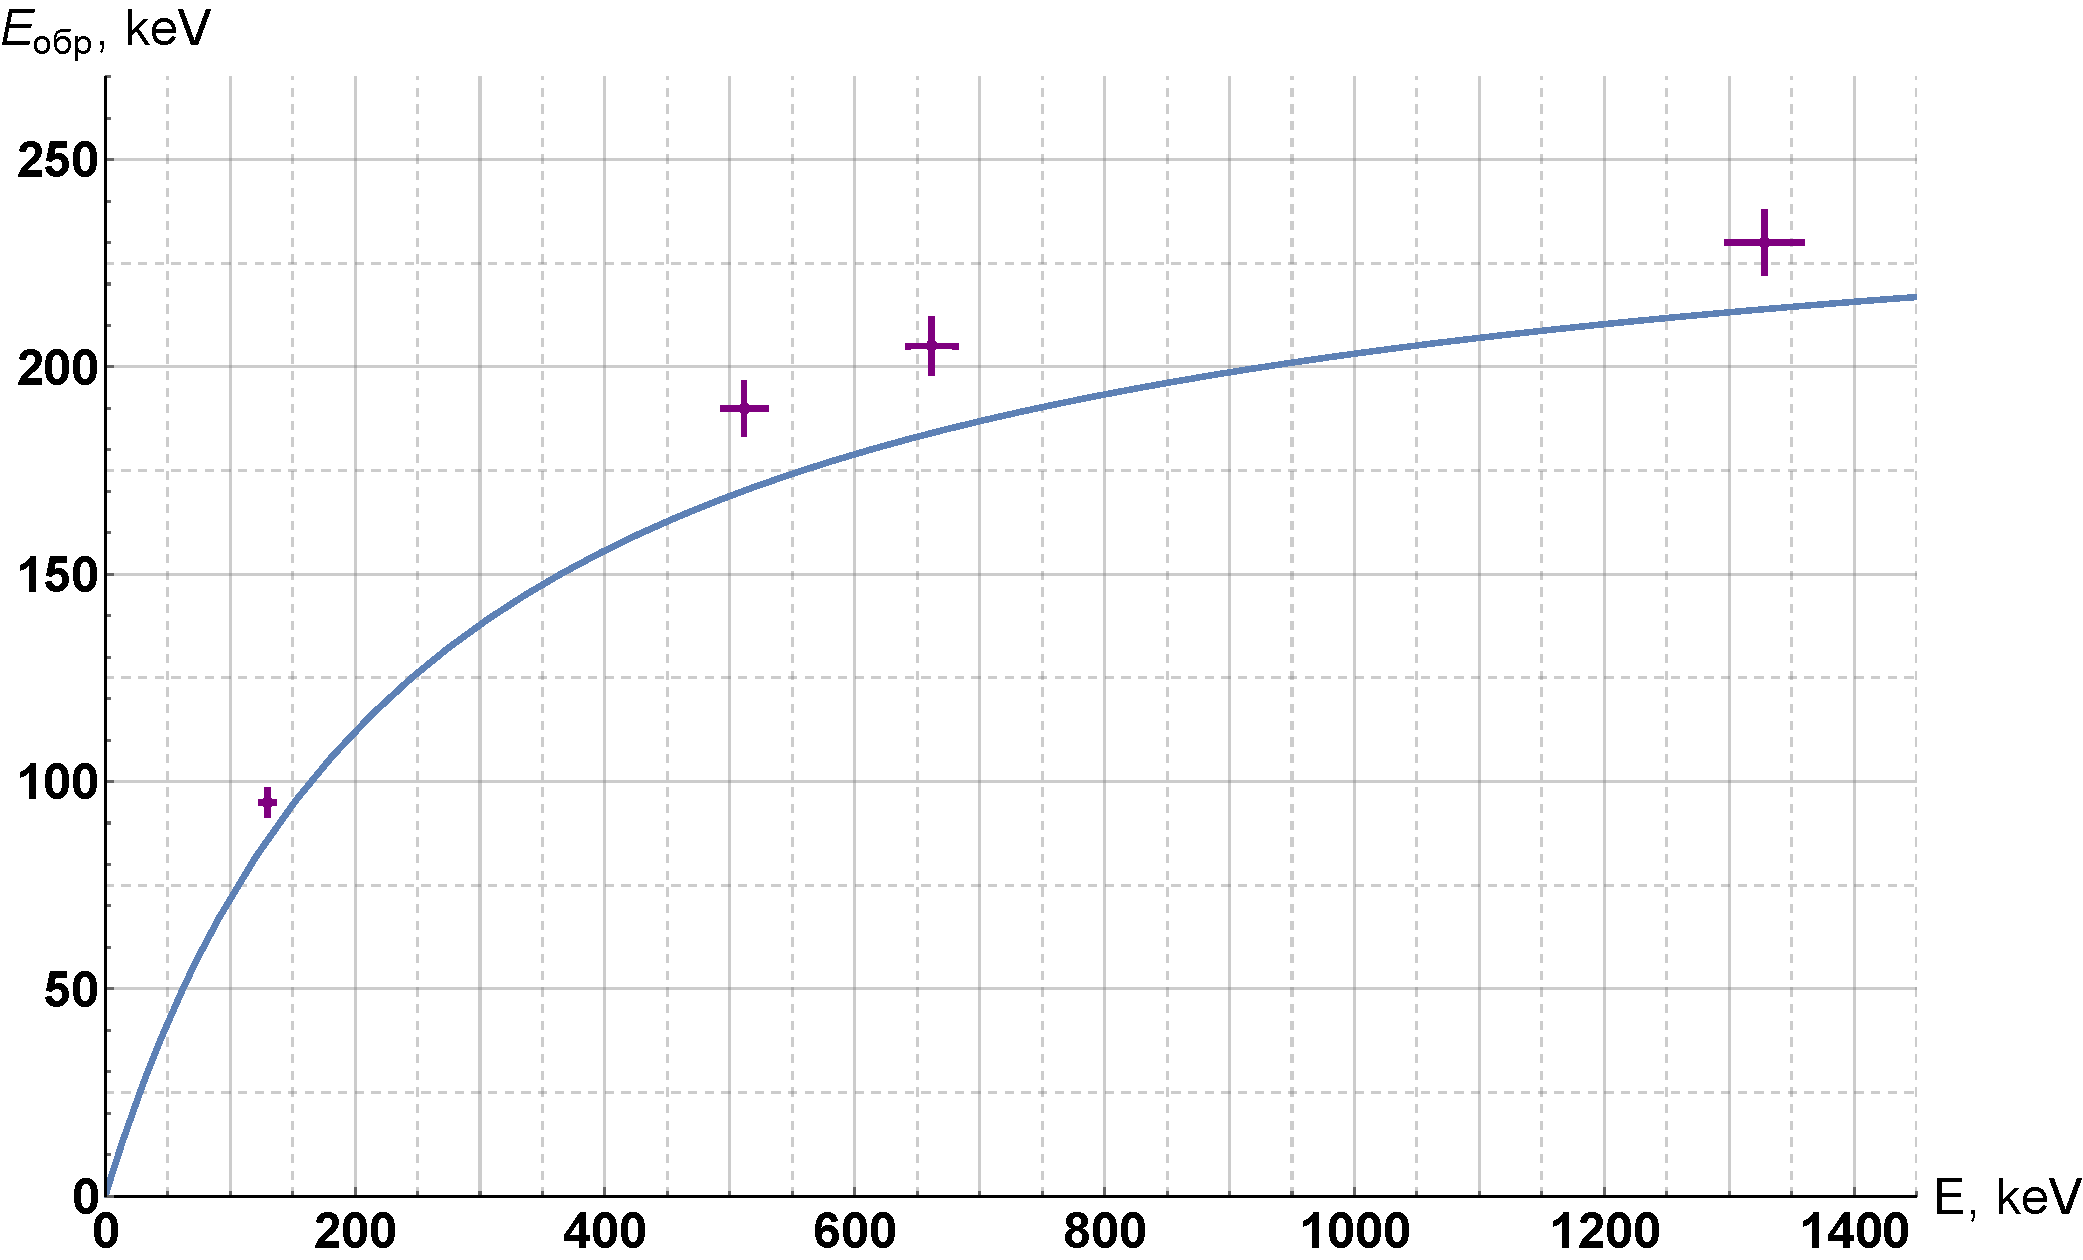
\includegraphics[width=10cm]{src/ee.pdf}
	\caption{Пики обратного рассеяния}
\end{figure} 

Заметим, что на наших графиках (для натрия, цезия, кобальта и европия) в левой части спектра присутствует узкий (небольшой и широкий для европия) пик, соответствующий энергии порядка $ E_x \simeq 80 $ кэВ. Это соответствует характеристическому излучению из свинца, служащего защитой спектрометра от внешнего излучения. 

Пронаблюдав на осциллографе изображение импульсов с ФЭУ, оценим величины $ \tau_0 \simeq 0,6 $~мкс~---~характерное время высвечивания для ФЭУ, и постоянную времени $ RC \simeq 35 $ мкс. Это было оценено по передним и задним фронтам импульсов соответственно. 


\clearpage
    
\section*{Вывод}

В ходе работы после калибровки прибора были сняты спектры образцов $^{22}$Na,  $^{60}$Cо,  $^{137}$Cs, $^{241}$Am, $^{152}$Eu, а также исследован спектр неизвестного образца и определен его состав ($^{137}$Cs). В спектрах были исследованы пики, соответствующие следующим взаимодействиям гамма-квантов с веществом:

\begin{itemize}
    \item фотоэффект (пики полного поглощения)
    \item эффект Комптона (характерное распределение энергий в спектре, оканчивающееся комптоновским краем)
    \item обратное рассеяние (пики обратного рассеяния)
    \item аннигиляция позитронов (пик 511 keV в спектре натрия, по которому проводилась калибровка)
\end{itemize}

Все значения энергии, опеределённые по спектрам, практически совпадали с табличными и расчётными. \par

Также была проверена линейная зависимость квадрата спектрального разрешения прибора от величины, обратной энергии полного поглощения.

\vfill
    
\begin{thebibliography}{9}
	\bibitem{max} \emph{Лабораторный практикум по общей физике. В 3 томах. Том 3. Квантовая физика: учебное пособие} под ред. Ю. М. Ципенюка
\end{thebibliography}

\end{document}
